\documentclass{article}

\usepackage{tikz}
\usetikzlibrary{automata, positioning}
\begin{document}
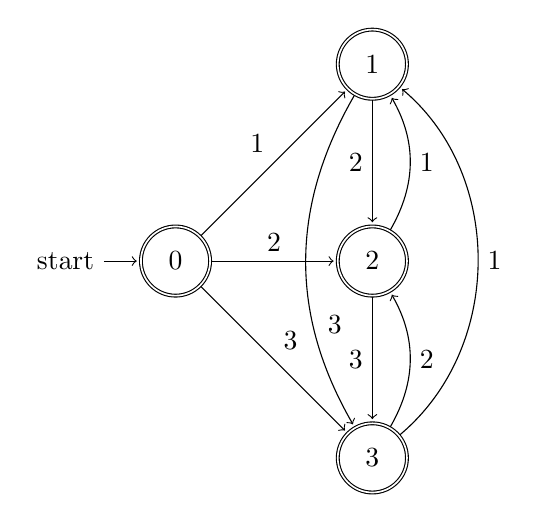
\begin{tikzpicture}[shorten >= 1pt, node distance = 2.5cm, on grid, auto]
  \node[state, initial, accepting] (0) {0};
  \node[state, accepting] (2) [right=of 0] {2};
  \node[state, accepting] (1) [above=of 2] {1};
  \node[state, accepting] (3) [below=of 2] {3};
  \path[->]
    (0) edge node {1} (1)
        edge node {2} (2)
        edge node {3} (3)
    (1) edge node [left] {2} (2)
        edge [bend right] node [near end] {3} (3)
    (2) edge node [left] {3} (3)
        edge [bend right] node [right] {1} (1)
    (3) edge [bend right] node [right] {2} (2)
        edge [bend right=50] node [right] {1} (1);
\end{tikzpicture}
\end{document}
